
%%%%%%%%%%%%%%%%%%%%%%%%%%%%%%%%%%%%%%%%%%%%%%
This section describes the features of the WOS Backend and how it interacts with the different ESDM components to perform the read and write activity on behalf of the user applications.

\subsection{Logical View}

The DDN WOS object storage solution (see \Cref{WOS background}) represents a storage system architecture which manages data as objects, automatically storing files in the cloud in a geographically agnostic manner. Each object is stored with a unique OID that is used to retrieve the related data, delete them or verify the existence.
The logical view for interactions between ESDM and Clovis/Mero is illustrated in \Cref{fig:WOS backend logical view}.

To interact with the WOS cluster, DDN provides API for C++, JAVA and Python languages and an HTTP Restful interface; in particular operations as Put, Get, Delete, Exists, Reserve and PutOID are allowed in blocking and non-blocking form.

\begin{figure}
	\centering
	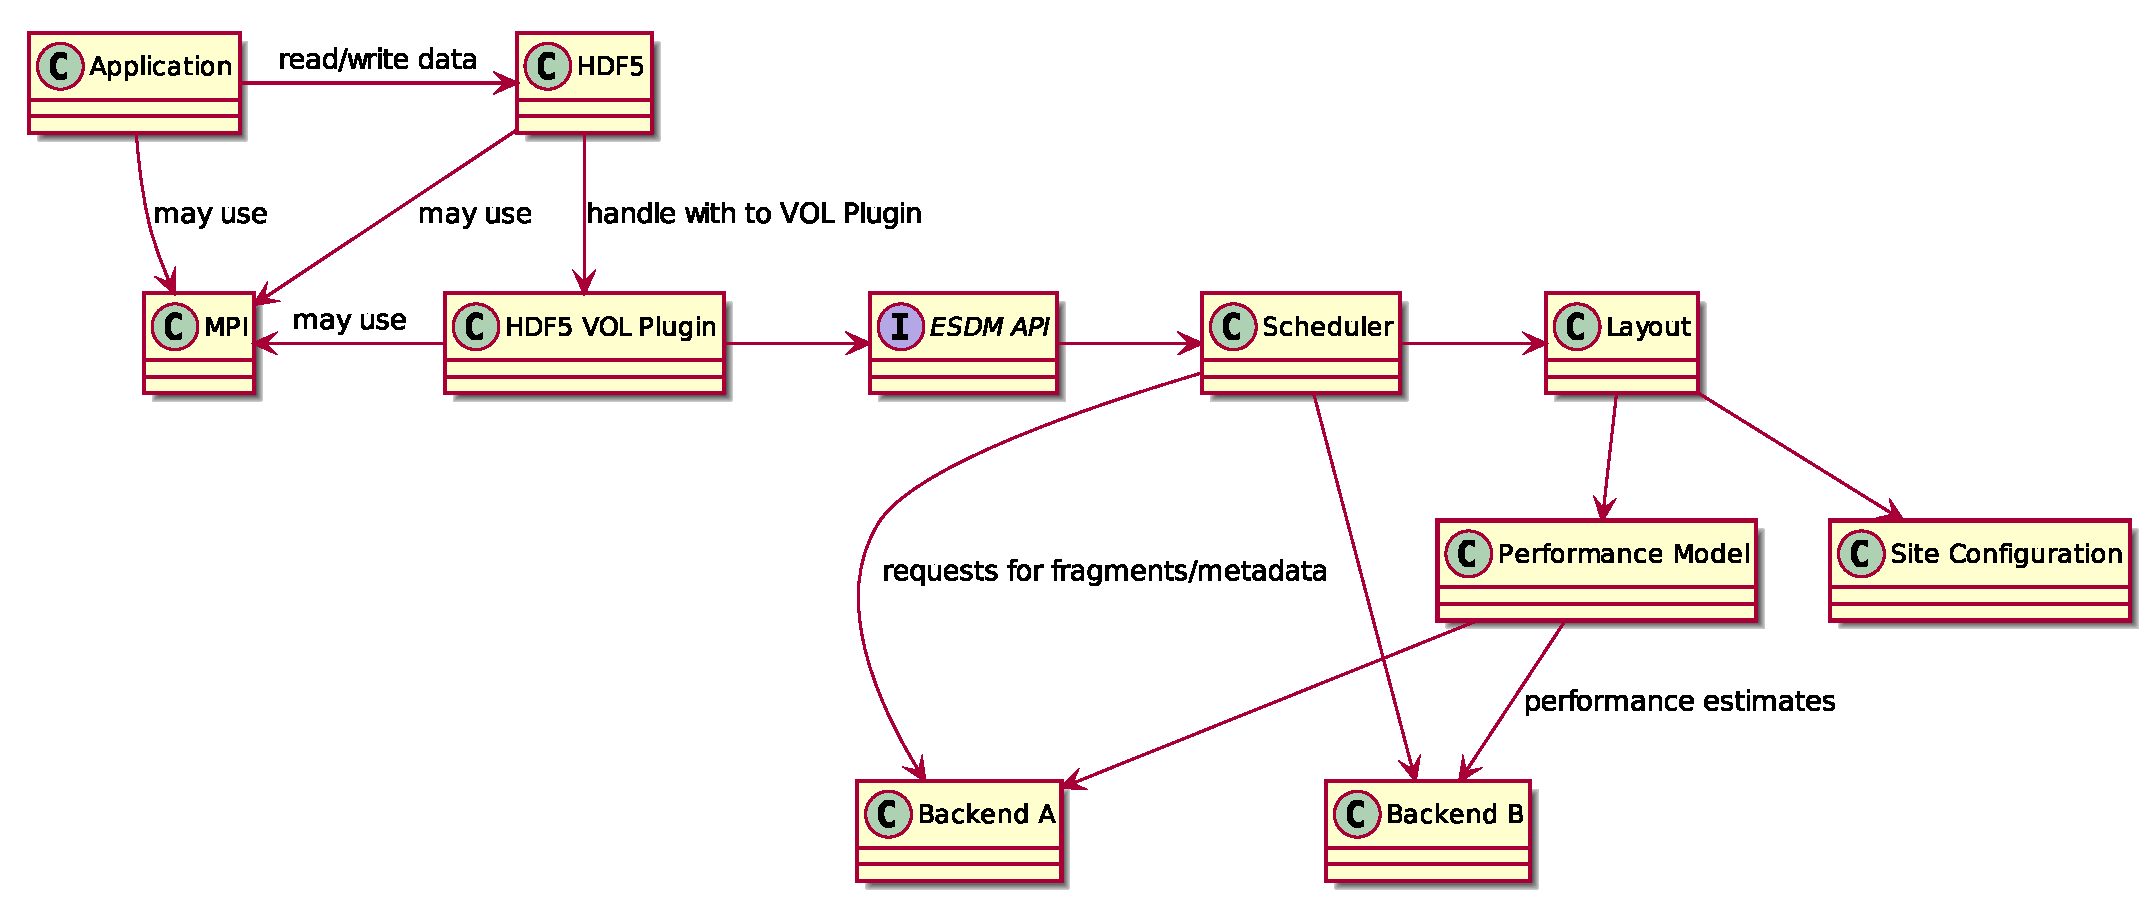
\includegraphics[width=\linewidth]{esdm-backends/WOS/logical.eps}
	\caption{Logical view to the WOS backend. I/O requests arrive through the ESDM API. The layout component provides a fragmentation based on site configuration and performance model. As a result, actual I/O requests are processed by the progress component which calls the backends providing the needed metadata. The backends and the datatype components work together to convert data according to what is required.}
	\label{fig:WOS backend logical view}
\end{figure}

\paragraph{Writing data:}
The following sequence extends the Use-Case description for general writing (see \Cref{uc: independent write}).
A sequence diagram for the chain of events is provided by \Cref{fig:WOS backend sequence write}.

\begin{itemize}
	\item Progress consults layout about the choice of the most suitable backend and the proper fragmentation.
	\item Progress sends data to WOS backend.
	\item WOS backend accepts the incoming data properly managing the correct datatype conversion.
	\item WOS backend creates a new WOS Object.
	\item WOS Storage returns the corresponding Object Identifier (OID)
	\item WOS backend saves data to the WOS Storage
	\item WOS backend returns the OID to the Progress module
\end{itemize}

\begin{figure}
	\centering
	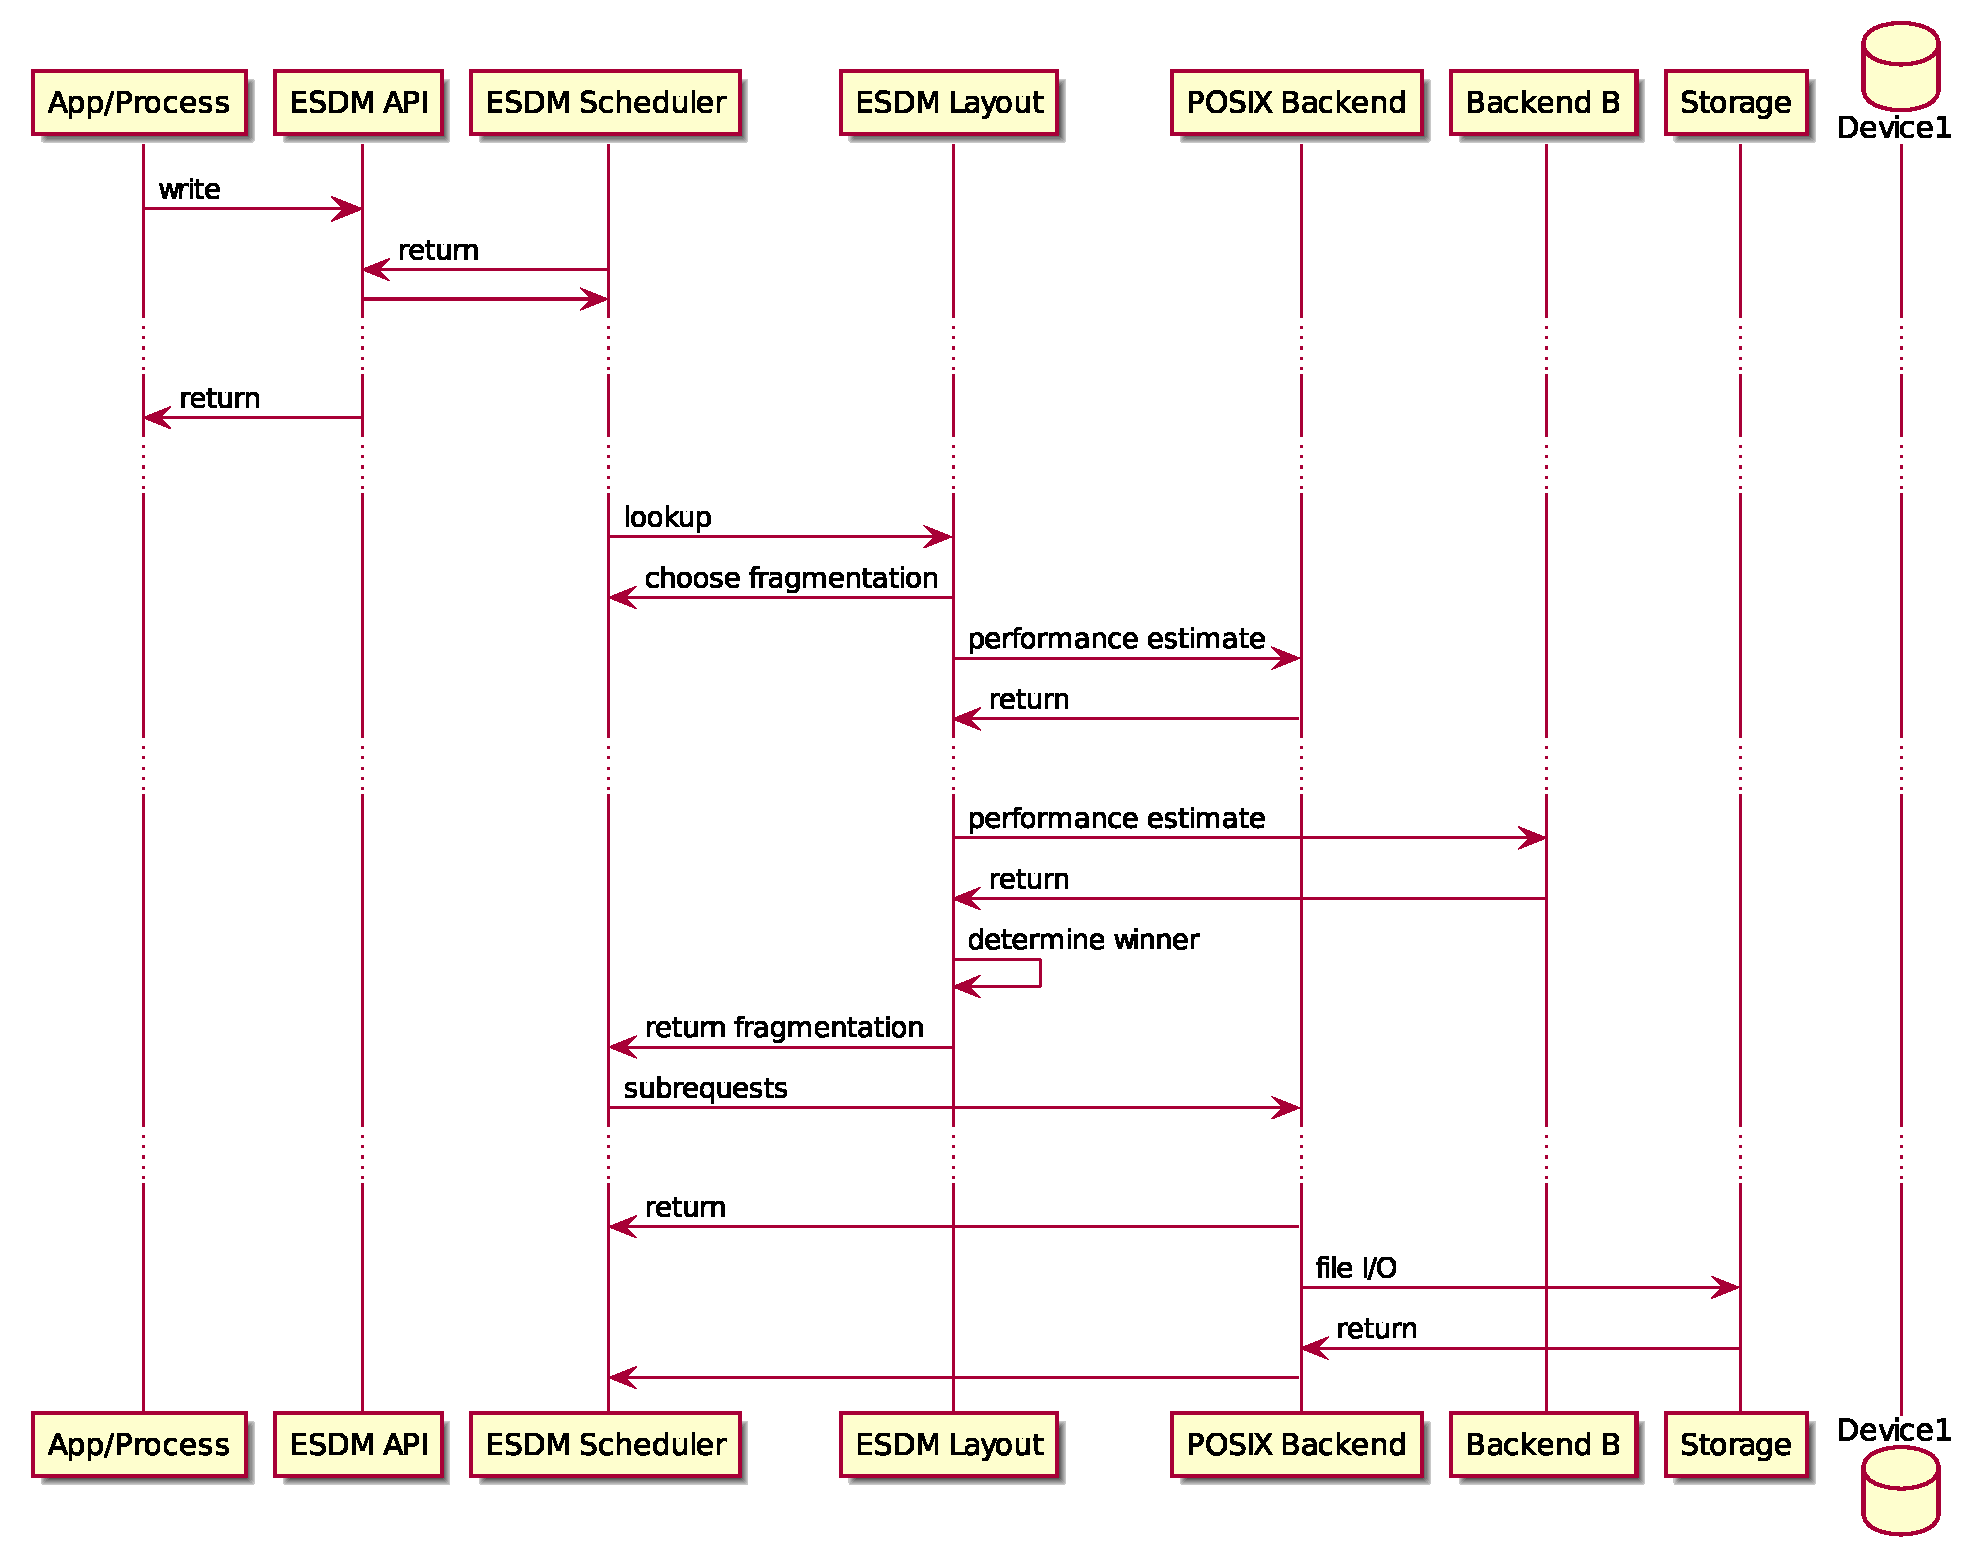
\includegraphics[width=\linewidth]{esdm-backends/WOS/sequence_write.eps}
	\caption{WOS backend sequence write}
	\label{fig:WOS backend sequence write}
\end{figure}

\paragraph{Reading data:}
The following sequence extends the Use-Case description for general reading (see \Cref{uc: independent read}).
A sequence diagram for the chain of events is provided by \Cref{fig:WOS backend sequence read}.

\begin{itemize}
	\item Progress and Layout work together to eventually split the request into multiple subrequests, one for each fragment to retrieve
	\item Layout collects the needed metadata related to the fragments to retrieve
	\item Progress forward the request to the WOS backend; multiple requests could be sent in parallel
	\item WOS backend retrieves data from the WOS Storage based on OID (Object Identifier)
	\item WOS backend performs the needed datatype conversion
	\item WOS Backend returns data
	\item Data is provided to the application
\end{itemize}

It is worth noting that WOS storage manages data in binary format only: no information about data type needs to be passed to the storage for writing or reading. The WOS backend, the Layout and the Datatype perform the required communications for properly managing the different data types.

\begin{figure}
	\centering
	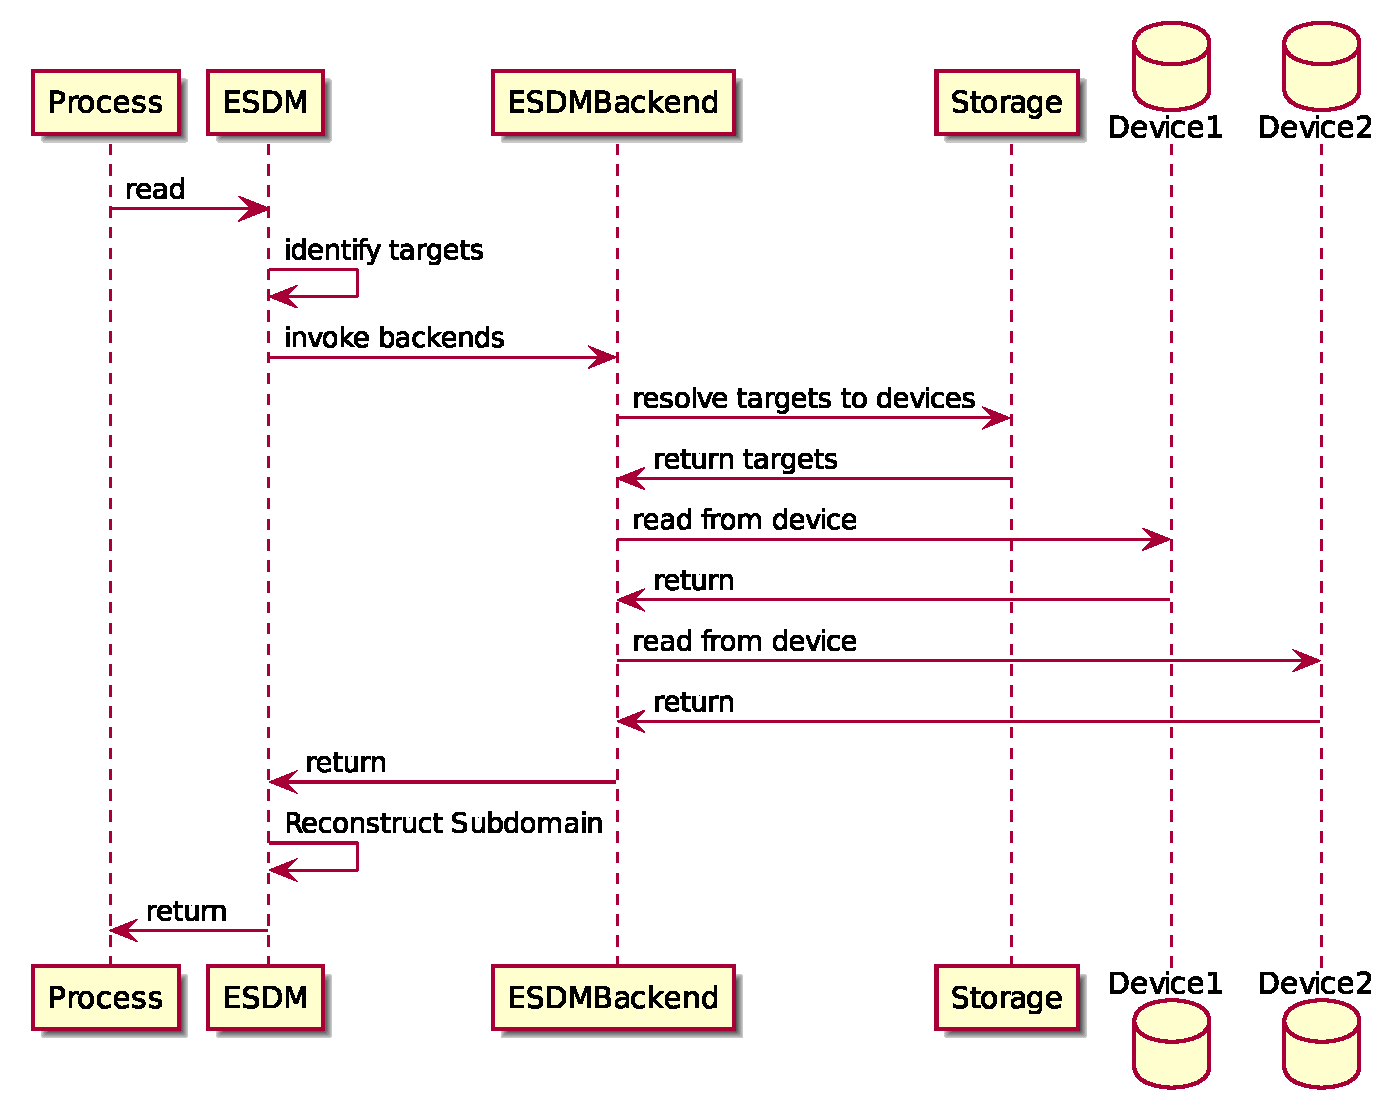
\includegraphics[width=\linewidth]{esdm-backends/WOS/sequence_read.eps}
	\caption{WOS backend sequence read}
	\label{fig:WOS backend sequence read}
\end{figure}

\paragraph{Lookup:}
WOS Objects relies on the concept of Object Identifier: each Object is associated with a unique OID and once used an OID cannot be reassigned. OID is the identifier needed by the application for accessing the object and retrieving its data. As stated before, objects are saved into the storage in binary format (for instance mapped as a pointer to a \textit{void} variable in C++ code): user applications need to provide the proper mapping to the final datatype.

Fragments are associated with WOS Objects: the lookup phase is allowed by using the correct OID stored in the metadata backend and provided to the WOS backend to perform the association with the related object. 


%%%%%%%%%%%%%%%%%%%%%%%%%%%%%%%%%%%%%%%%%%%%%%
\subsection{Process View}

\textbf{Progress Component} The progress component is responsible for managing the interactions with the WOS backend, in terms of synchronous and asynchronous call handling. It communicates with the ESDM\textunderscore WOS\textunderscore Service exchanging the proper information about data transferring, metadata management and status of the processes.
\Cref{fig:WOS backend process view} illustrates the processes and services related to the WOS backend.

\textbf{ESDM\textunderscore WOS\textunderscore Service} The ESDM\textunderscore WOS\textunderscore Service represents the middleware between the progress component and the WOS System Storage. It accepts requests incoming from the progress component concerning data and/or metadata management, and fragments read and write. The ESDM\textunderscore WOS\textunderscore Service can translate such requests into WOS Cluster call which finalises the operations to the WOS Storage. As supported by the WOS architecture, the ESDM\textunderscore WOS\textunderscore Service can manage blocking and non-blocking calls on behalf of the progress component.\\

\textbf{WOS Cluster} The WOS Cluster represents the remote host pool and services able to accept, manage and finalise the incoming requests/data from the ESDM\textunderscore WOS\textunderscore Service. It hosts the WOS Storage and physically handles the retrieval of the requested information triggered by the higher level applications and services.

\begin{figure}
	\centering
	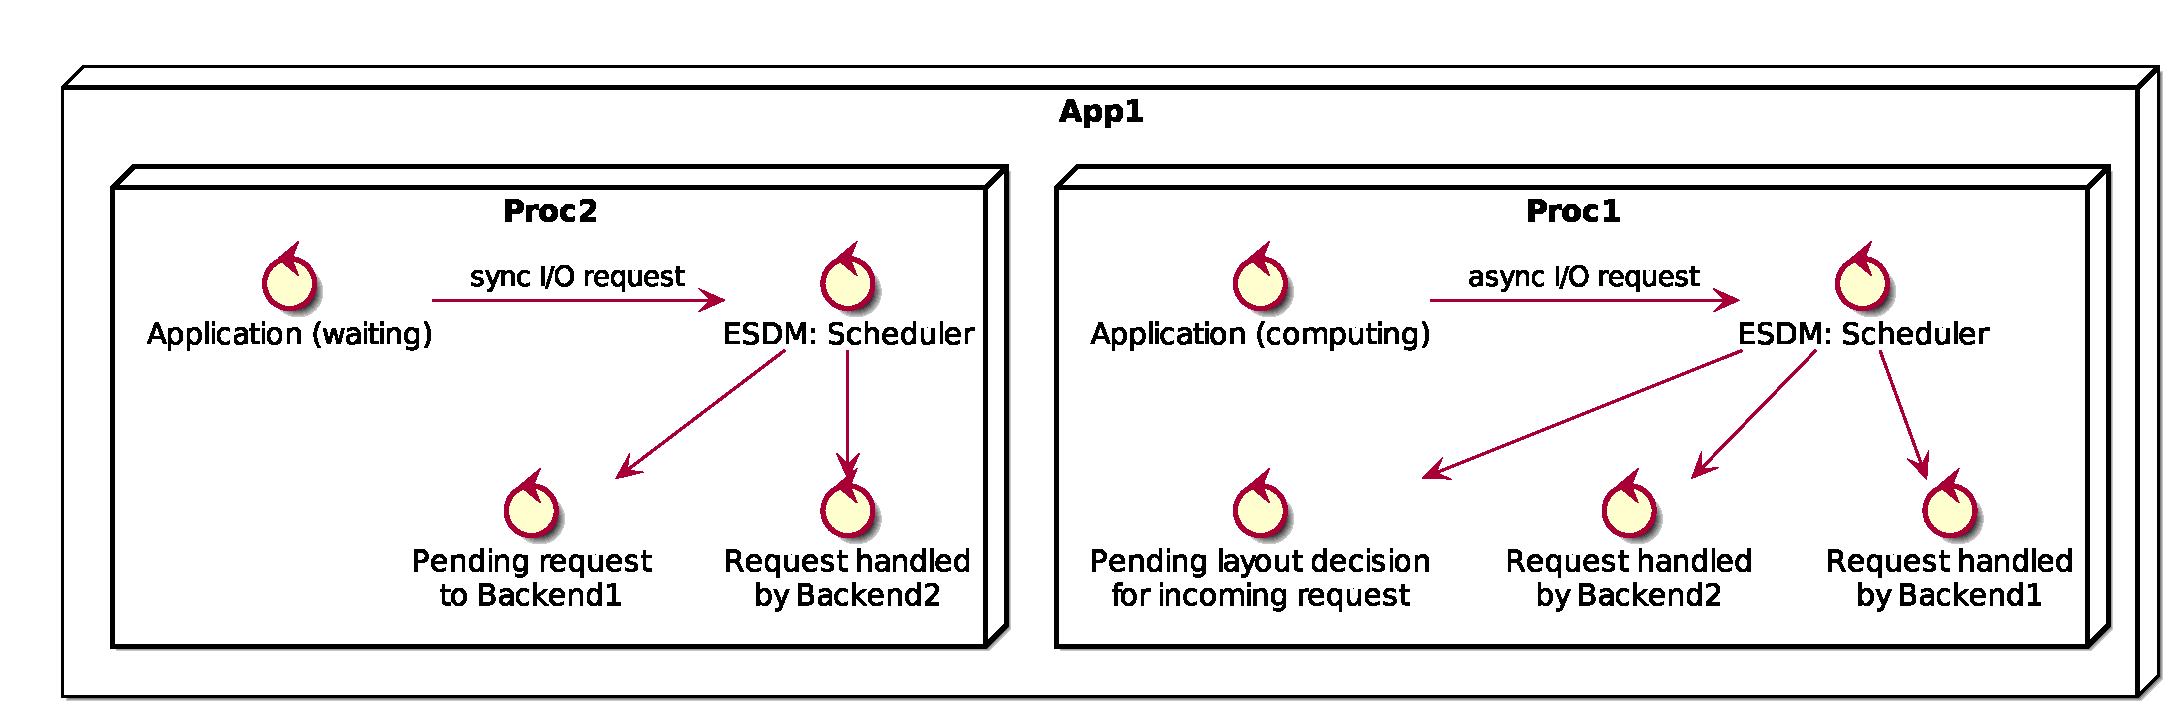
\includegraphics[width=\linewidth]{esdm-backends/WOS/process.eps}
	\caption{Overview of processes and entities involved in the interaction with the WOS backend}
	\label{fig:WOS backend process view}
\end{figure}


%%%%%%%%%%%%%%%%%%%%%%%%%%%%%%%%%%%%%%%%%%%%%%
\subsection{Development View}

The interactions between the ESD middleware and the WOS Storage relies on a WOS interface managed by the ESDM WOS Service. Such component represents the link between the ESD middleware and the WOS Storage and Services providing the proper interfaces for interacting with the WOS cluster. It can handle requests for synchronous and asynchronous operations exploiting the blocking and non-blocking form of the WOS API calls. Tailored to support the ESD middleware functionalities, it hides the internal features of WOS and manages the translation between WOS and ESD datatypes.  


%%%%%%%%%%%%%%%%%%%%%%%%%%%%%%%%%%%%%%%%%%%%%%
\subsection{Physical View}

WOS Storage System relies on a pool of services and daemons to properly manage the incoming read and write requests as is illustrated in \Cref{fig:WOS backend physical view}.
Such services can handle the entire WOS infrastructure from a hardware and software point of view, accepting and dispatching the requests for getting/putting data (in a blocking and non-blocking form) to the proper node instance inside the cloud and to the related storage. 
WOS configuration allows the administrator to define zones and policies for defining different groups of nodes associated with different rules and objects distribution on the physical storage.
In addition, an administrator can configure replica policy rules which will be automatically managed by the WOS cloud system. 
In this perspective, ESD middleware relies on the WOS configuration and policies for the management of the distribution of the objects among the nodes of the cluster and the physical mapping of the data on the disks. 
At a higher level, ESD middleware can exploit the WOS backend functionalities to customise the distribution of the objects.


\begin{figure}
	\centering
	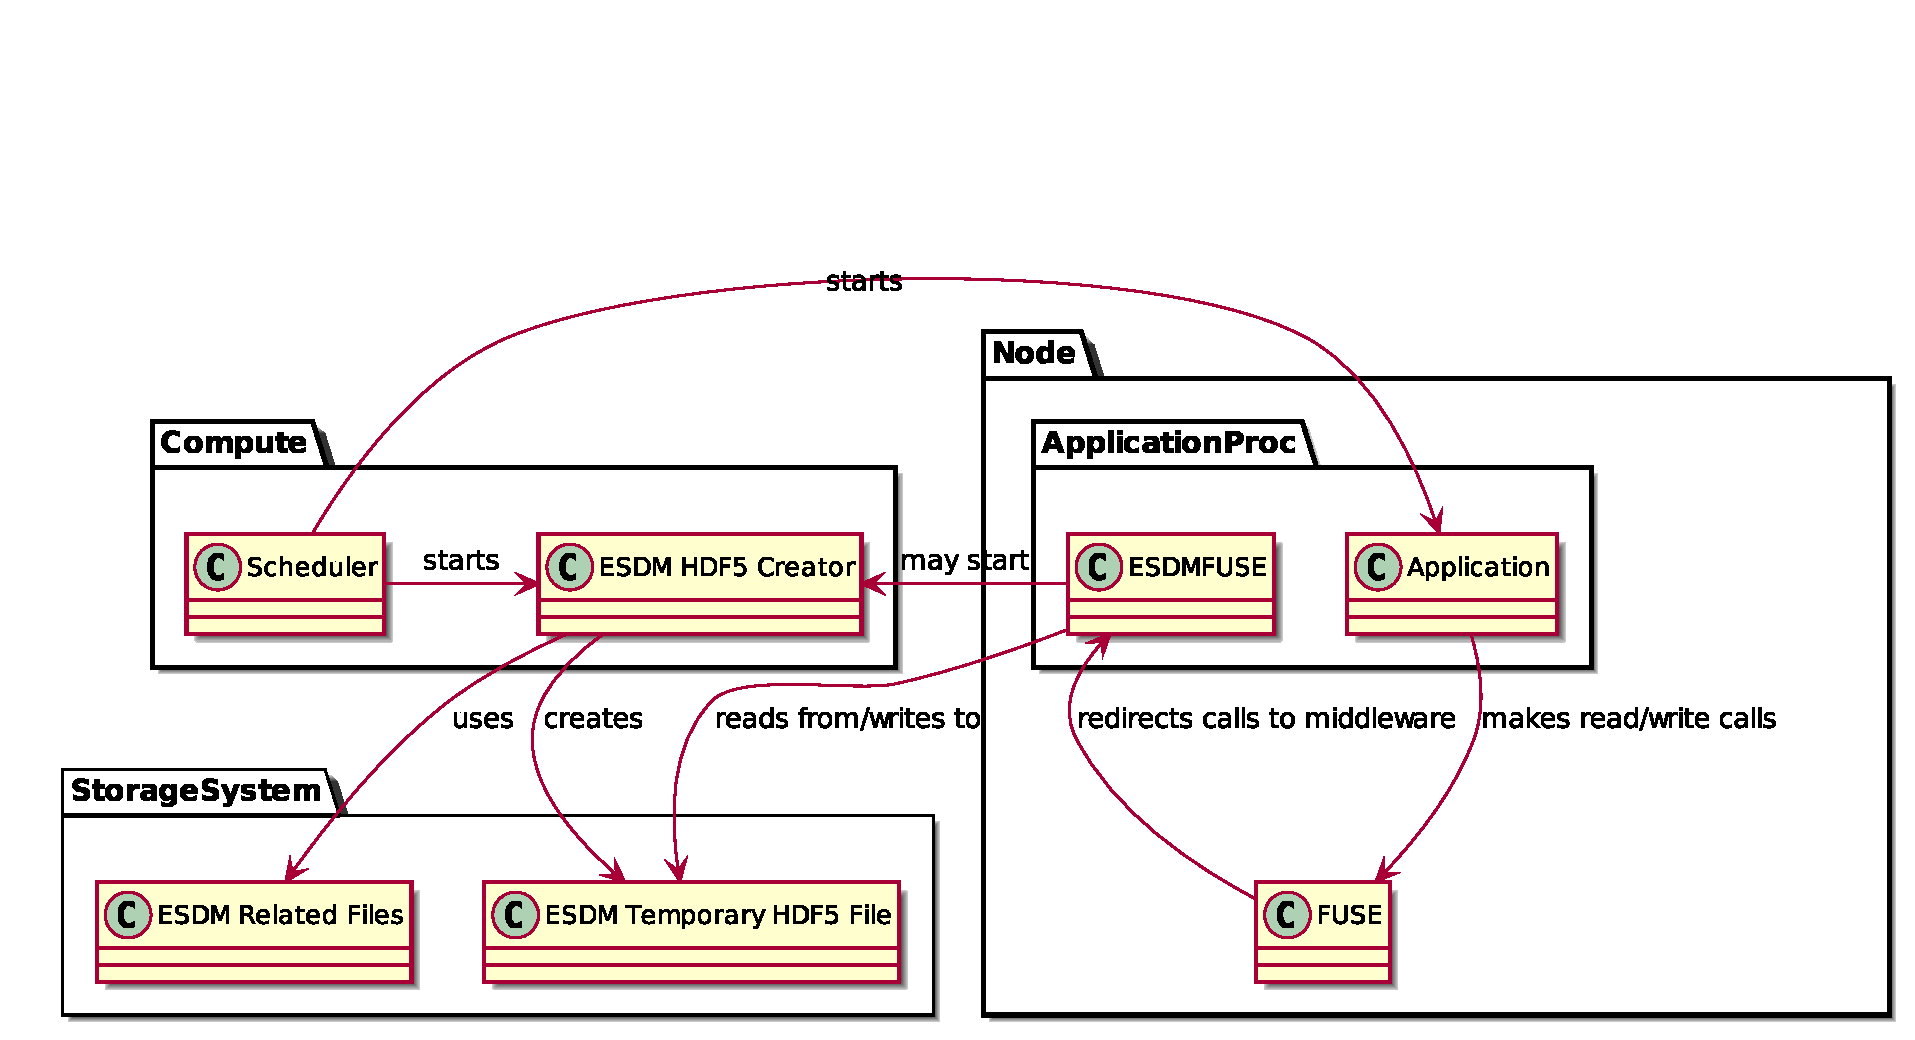
\includegraphics[width=\linewidth]{esdm-backends/WOS/physical.eps}
	\caption{WOS backend physical view}
	\label{fig:WOS backend physical view}
\end{figure}



